\documentclass{patmorin}
\listfiles
\usepackage{pat}
\usepackage{paralist}
\usepackage[T1]{fontenc}
\usepackage[utf8]{inputenc}
\usepackage{bbm}  % needed for \mathbbm{1}
% \usepackage{logix}
\usepackage{halloweenmath}
\usepackage{stmaryrd}

\usepackage{todonotes}
\usepackage{tcolorbox}
\usepackage{booktabs}
\usepackage{multirow}
\usepackage{comment}

\usepackage{thm-restate}


% etoolbox allows for robust commands that don't need \protect, e.g.
% \newrobustcmd{\onesub}{\mathord{\includegraphics{figs/one-sub}}}
% \subsection{Approximate Voronoi Diagrams in $G^{\onesub}_k$}
\usepackage{etoolbox}

% david proposes the following additions
\renewcommand{\ge}{\geqslant}
\renewcommand{\le}{\leqslant}
\renewcommand{\geq}{\geqslant}
\renewcommand{\leq}{\leqslant}

\newcommand{\david}[1]{{\color{orange} David: #1}}
\newcommand{\vida}[1]{{\color{DarkGreen} Vida: #1}}
\newcommand{\pat}[1]{\textcolor{Blue}{Pat: #1}}
\newcommand{\gwen}[1]{\textcolor{Purple}{Gwen: #1}}
\newcommand{\piotr}[1]{\textcolor{red}{Piotr: #1}}

% \numberwithin{equation}{lem}


\newenvironment{clmproof}{\noindent\emph{Proof of Claim:}}{\hfill\rule{1ex}{1ex}}

\usepackage[longnamesfirst,numbers,sort&compress]{natbib}

\usepackage[mathlines]{lineno}
\setlength{\linenumbersep}{2em}
% \linenumbers
% \rightlinenumbers
% \linenumbers
\newcommand*\patchAmsMathEnvironmentForLineno[1]{%
 \expandafter\let\csname old#1\expandafter\endcsname\csname #1\endcsname
 \expandafter\let\csname oldend#1\expandafter\endcsname\csname end#1\endcsname
 \renewenvironment{#1}%
    {\linenomath\csname old#1\endcsname}%
    {\csname oldend#1\endcsname\endlinenomath}}%
\newcommand*\patchBothAmsMathEnvironmentsForLineno[1]{%
 \patchAmsMathEnvironmentForLineno{#1}%
 \patchAmsMathEnvironmentForLineno{#1*}}%
\AtBeginDocument{%
\patchBothAmsMathEnvironmentsForLineno{equation}%
\patchBothAmsMathEnvironmentsForLineno{align}%
\patchBothAmsMathEnvironmentsForLineno{flalign}%
\patchBothAmsMathEnvironmentsForLineno{alignat}%
\patchBothAmsMathEnvironmentsForLineno{gather}%
\patchBothAmsMathEnvironmentsForLineno{multline}%
}



% Taken from
% https://tex.stackexchange.com/questions/42726/align-but-show-one-equation-number-at-the-end
\newcommand\numberthis{\addtocounter{equation}{1}\tag{\theequation}}

\definecolor{brightmaroon}{rgb}{0.76, 0.13, 0.28}
\definecolor{linkblue}{rgb}{0, 0.337, 0.227}
\newcommand{\defin}[1]{\emph{\textcolor{brightmaroon}{#1}}}
\makeatletter
\def\mathcolor#1#{\@mathcolor{#1}}
\def\@mathcolor#1#2#3{%
  \protect\leavevmode
  \begingroup
    \color#1{#2}#3%
  \endgroup
}
\makeatother
\newcommand{\mathdefin}[1]{\mathcolor{brightmaroon}{#1}}
% \newcommand{\mathdefin}[1]{\color{brightmaroon}#1}}
\setlength{\parskip}{1ex}

% Document-specific commands and math operators
\DeclareMathOperator{\tw}{tw}
\DeclareMathOperator{\pw}{pw}
\DeclareMathOperator{\bw}{bw}
\DeclareMathOperator{\td}{td}
%\DeclareMathOperator{\rtw}{rtw}
\DeclareMathOperator{\diam}{diam}
\DeclareMathOperator{\mindist}{min-dist}
\DeclareMathOperator{\dist}{dist}
\DeclareMathOperator{\ld}{ld}
\DeclareMathOperator{\polylog}{polylog}
\DeclareMathOperator{\evol}{Evol}
\DeclareMathOperator{\ivol}{Ivol}
\DeclareMathOperator{\tvol}{Tvol}
\newcommand{\NN}{\mathbb{N}}
\newcommand{\GG}{\mathcal{G}}

\title{\MakeUppercase{\boldmath Geometric Intersection Graphs and Blowups of Bounded Pathwidth Graphs}}

%\title{\MakeUppercase{\boldmath Planar graphs are contained in $\tilde{O}(\sqrt{n})$-blowups of fans}}

%Fan-Partitions of Planar Graphs (and Beyond)  \newline by Local Sparsification and Volume-Preserving Embeddings}}

\author{TBD}
 % Vida Dujmovi{\'c}\,\footnote{School of Computer Science and Electrical Engineering, University of Ottawa, Ottawa, Canada (\texttt{vida.dujmovic@uottawa.ca}). Research supported by NSERC and a University of Ottawa Research Chair.}
 % \qquad
 % Gwena\"el Joret\footnote{D\'epartement d'Informatique, Universit\'e libre de Bruxelles, Belgium ({\tt gwenael.joret@ulb.be}). G.\ Joret is supported by the Belgian National Fund for Scientific Research (FNRS) and by the Australian Research Council.}
 % \qquad
 % Piotr Micek\footnote{Department of Theoretical Computer Science, Jagiellonian University, Kraków, Poland (\texttt{piotr.micek@uj.edu.pl}). Research supported
 % the National Science Center of Poland under grant UMO-2018/31/G/ST1/03718 within the BEETHOVEN program.}
 % \qquad
 % Pat Morin\footnote{School of Computer Science, Carleton University, Ottawa, Canada (\texttt{morin@scs.carleton.ca}). Research supported by NSERC and the Ontario Ministry of Research and Innovation.}
 % \qquad
 % David~R.~Wood\footnote{School of Mathematics, Monash University, Melbourne, Australia (\texttt{david.wood@monash.edu}). Research supported by the Australian Research Council.}
 % }

\date{}


\begin{document}

\maketitle

\section{Introduction}

These are some notes about try to extend the following theorem of Alon from unit disks to arbitrary disks:

\begin{thm}[Alon]\label{alon}
  For every set $S$ of $n$ disjoint unit discs in the plane, there exists a direction $\alpha$ such that every line parallel to $\alpha$ intersects $O(\sqrt{n\log n})$ discs in $S$.
\end{thm}

One application of this result is that if $G$ is a unit disc intersection graph with maximum clique size $\omega$, then performing performing a line sweep with lines in direction $\alpha$, this gives an unit-interval graph that contains $G$ and has maximum clique size $O(\omega \sqrt{n\log n})$.  Variations of this for intersection graphs of discs whose radii can be covered by a bounded-size set of intervals of the form $[a,2a]$ show, for example, that such graphs are contained in $O(\omega\sqrt{n\log n})$-blowups for bounded pathwidth graphs, where the pathwidth depends only on the number of intervals needed to cover the radii of the discs.

Of course, \cref{alon} can't be extended to arbitrary sets of disjoint discs because the following arrangement of discs has a point $p$ such that every line that contains $p$ intersects at least $n/6$ of the discs.

\begin{center}
  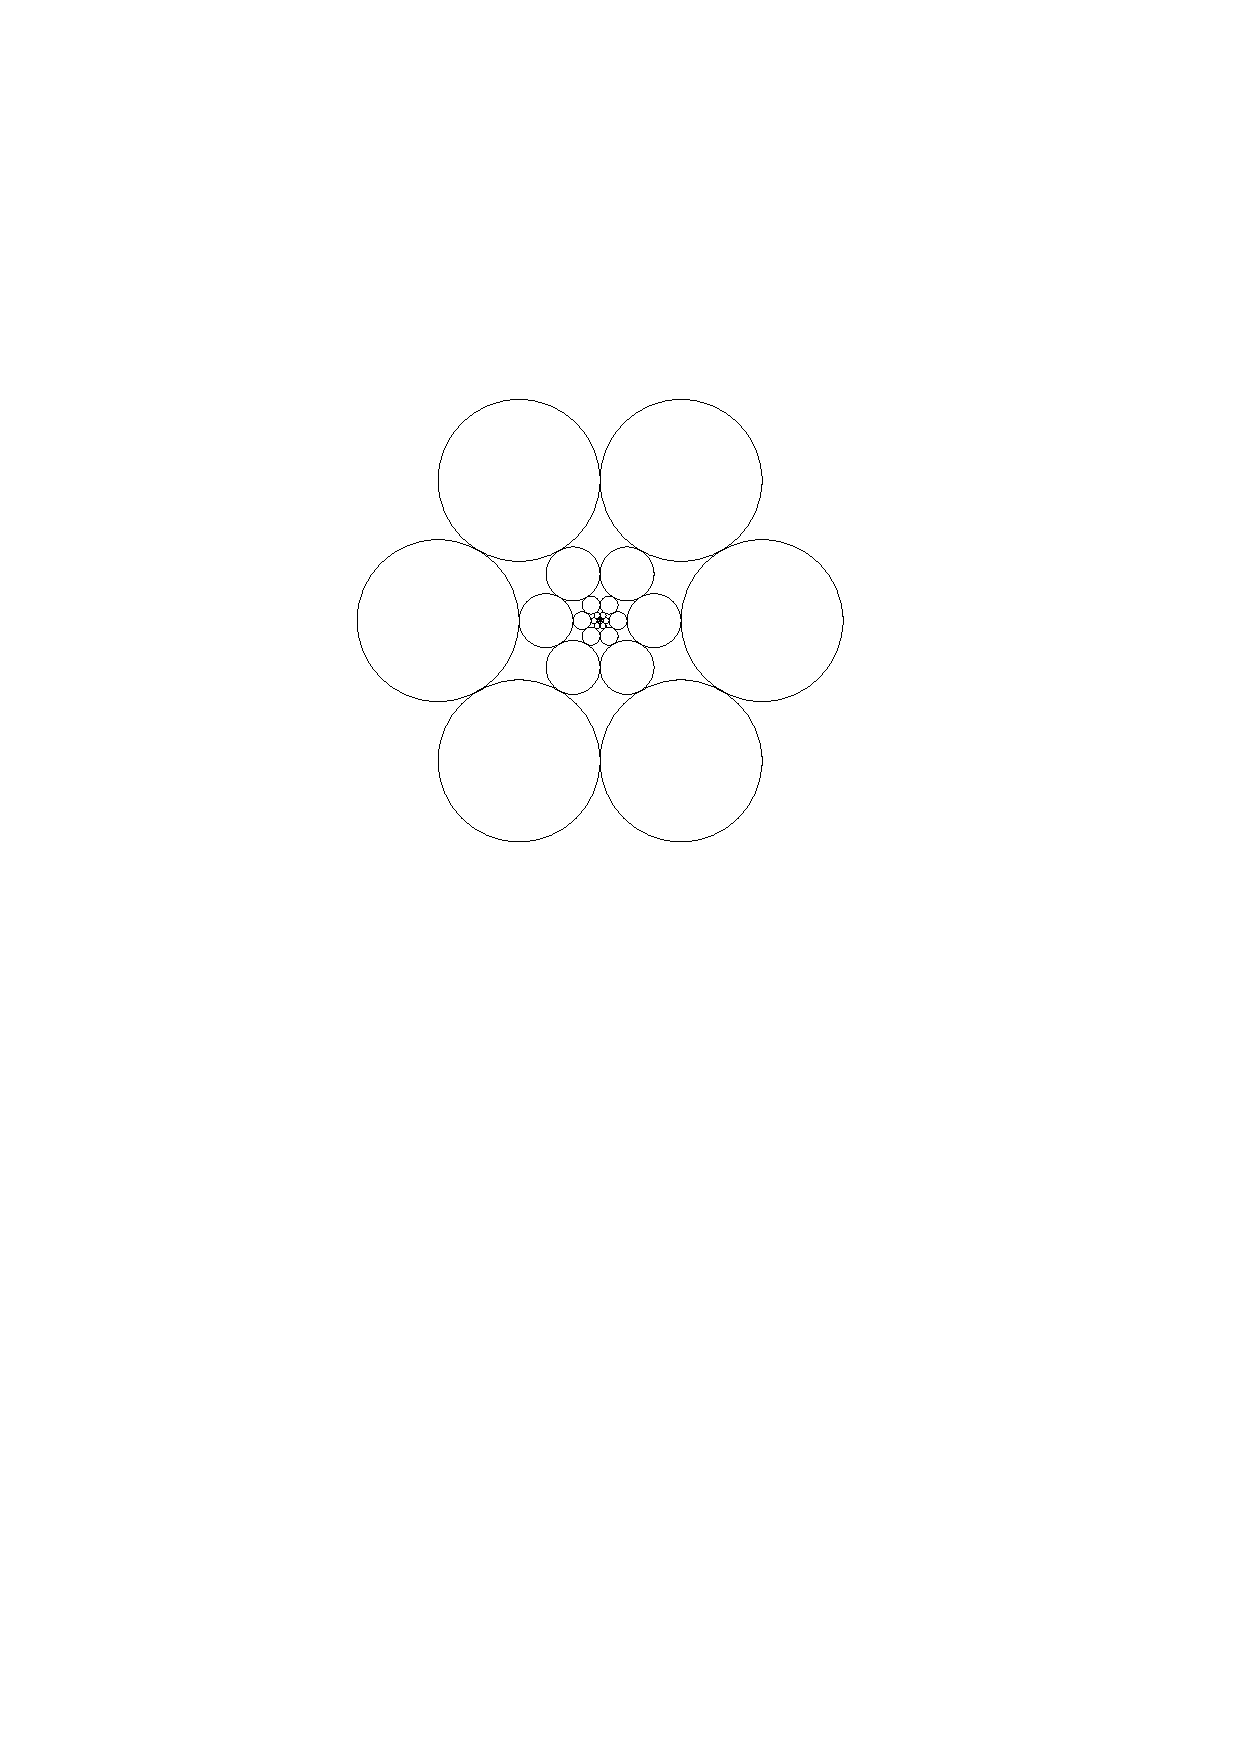
\includegraphics{figs/spider}
\end{center}

One possibility is to do a circle sweep instead. In the bad example above, choosing $p$ to be the center of the figure and sweeping with a circle centered at $p$ gives an interval graph representation with maximum clique size $12$.  In general there is not always a good $p$  If you construct two copies of the preceding example that are very far apart then $p$ will be so far from at least one of them that all circles centered at $p$ basically behave like parallel lines with respect to this copy.

Now that I write this, I see that this example also explains why what I discuss below can't work.  But, here is something I can prove that might help get rid of these kinds of configurations:

\begin{lem}
  Let $S$ be a set of $n$ disjoint circles and let $p$ be a point such that every line that contains $p$ intersects at least $k$ of the discs in $S$.  Then there exists a disc $D$ centered at $p$ that contains $\Omega(n)$ discs in $S$, that avoids $\Omega(n)$ discs in $S$ and whose boundary intersects $O(n/k)$ discs of $S$.
\end{lem}

\begin{proof}[Proof reminder]
  Map each disc in $S$ to an arc on $C(p,1)$ so that a line through $p$ intersects the disc if and only if it also intersects the corresponding arc.  Then, most of the arcs have length $\Omega(1/k)$, which means that the corresponding disc has radius at least $\Omega(1/k)$ times its distance from $p$.  For now, forget about the discs whose arcs have length less than $\epsilon/ k$.  Draw $2/k$ equally spaces rays out of $p$ and associate each disc in $S$ with the ray closest to its center.  Simple packing shows that each circle centered at $p$ intersects $O(1/k)$ discs of the discs we haven't eliminated (a constant number on each ray).  Now argue that the sequence of discs hit by each ray have exponentially increasing radii, so that there are  $\Omega(k)$ disjoint classes of distances of the form $[2^i,2^{i+1}]$.  One of these distances classes contains at most $n/k$ of the discs we forgot about.  Take $D$ to be any disc centered at $p$ whose radius is in this class.
\end{proof}

Not every bad example looks like this, though.  In the bad example, the discs come in three sets that each cover one third of the possible directions for a sweep line.  Each of these three sets can be translated and scaled arbitrarily and we will still get an example where, for each direction $\alpha$ there is a line paralell to $\alpha$ that intersects at least $n/3$ discs.


\paragraph{Old Hope:}

Instead, I would like to sweep with a circle whose radius $r$ grows while it's centers simultaneously moves at a speed of $1/2$.  Specifically, let $v$ be a (random) unit vector and let $p$ be any point in the plane, then for each $t\ge 0$, $C_t$ is the circle of radius $t$ centered at the point $p+tv/2$. Then $\{C_t: t\in[0,\infty)\}$ is a family of circles such that $C_{t'}$ contains $C_t$ in its interior for $t'\ge t\ge 0$.  If we can ensure that, for every $t$, $C_t$ intersects $O(\sqrt{n\log n})$ discs in $S$ then this would give a representation of the intersection graph of $S$ as an interval graph of maximum clique size $O(\sqrt{n\log n})$.  The hope is that the proof would also shed some insight into a representation of the intersection graph as the blowup for a bounded pathwidth graph.

The lemma below doesn't quite manage to do this.  It shows that, for a fixed $t$ and a randomly chosen unit vector $v$, $C_t$ intersets $O(\sqrt{n\log n})$ discs in $S$.  It's a theorem of the form, ``for each $t$ and nearly all $v$'' and I want a theorem of the form ``there exists some $v$ such that for all $t$''.  On the positive side, the theorem holds for any starting point $p$.  Maybe choosing $p$ carefully is important.  (Actually, no, see the comment above about two copies of the bad example.)


% Still, it's a start, and some of the things that come up in the proof already point towards things that are might be helpful in expressing the intersection graph as a blowup of a bounded pathwidth graph $G$.  For example, for each radius $t$ there are only $\tilde{O}(\sqrt{n})$ discs whose radius is larger than $t/\sqrt{n}$ that intersect $C_t$

\section{A First Lemma}

For a point $p\in\R^2$ and a real number $r$, let $\mathdefin{C(p,r)}:=\{q\in\R^2: d_2(p,q)=r\}$ be the circle of radius $r$ centered at $p$ and let $\mathdefin{D(p,r)}:=\{q\in\R^2: d_2(p,q)\le r\}$ be the closed disc of radius $r$ centered at $p$.  Let $\mathbf{0}:=(0,0)$ denote the origin.  For any $0\le r_1\le r_2$, let $\mathdefin{A(p,r_1,r_2)}:=D(p,r_2)\setminus D(p,r_1)\cup C(p,r_1)$ be the closed \defin{$(r_1,r_2)$-annulus} centered at $p$.

\begin{lem}
  Let $S$ be a set of $n$ pairwise-disjoint discs in the plane, and let $v\in C(\mathbf{0},1)$ be a uniformly random unit vector.  Then the expected number of disks in $S$ that intersect $C(v/2,1)$ is $O(\sqrt{n\log n})$.
\end{lem}

In the following proof, we repeatedly use the fact that, for concave increasing $f:\R_\ge 0\to\R$ and non-negative numbers $n_1,\ldots,n_k$ that sum to $n$, the sum $\sum_{i=1}^k f(n_i)$ is maximized when $n_1=\cdots=n_k=n/k$.  That is, $\sum_{i=1}^k f(n_i) \le k\,f(n/k)$.  In particular, we use this for $f(x)=\sqrt{x}$, in which case $\sum_{i=1}^k \sqrt{n_i}\le k\sqrt{n/k}=\sqrt{kn}$.

\begin{proof}
  The circle $C_i:=C(v/2,1)$ is contained in the disc $D:=(\mathbf{0},3/2)$, so we may assume that every disc in $S$ intersects $D$.  Since the discs in $S$ are pairwise disjoint, a standard packing argument implies that the number of discs of radius at least $1/\sqrt{n}$ that intersect $C(v/2,1)$ is $O(\sqrt{n})$. Therefore, we assume that all discs in $S$ have radius at most $1/\sqrt{n}$.

  For any integer $i\ge 1$, let $r_i=2^{-i}$ and let $S_i$ be the set of discs in $S$ whose radius is in the interval $(r_i,2r_i]$. For each $i\ge 1$, let $n_i:=|S_i|$. Fix some disc $B\in S_i$ with center $c$.  If $B$ intersects $C(v/2,1)$, then $v/2$ is contained in the annulus $A(c,1+2r_i,1-2r_i)$.  Some trigonometry and the inequality $1-\cos(\alpha)\le \alpha^2$ shows that the intersection of $C(\mathbf{0},1/2)$ with $A(c,1+2r_i,1-2r_i)$ is the union of (at most 2) circular arcs, each of length $\Omega(r_i)$ and having total length  $O(\sqrt{r_i})$. Therefore, the probability that $B$ intersects $C(v/2,1)$ is $O(\sqrt{r_i})$.

  % Therefore, the expected number of discs in $S$ of radius at most $r_i$ that intersect $C(v/2,1)$ is $O(n\sqrt{r_i})$.  This quantity is $O(\sqrt{n})$ for $r_i\le 2/n$, so we assume that all discs in $S$ have radius at least $1/n$.  In particular, $S_i$ is empty for all $i \ge \log_2 n$.\todo{Is this necessary?}

  We now push this argument further to consider a set of disks in $S_i$ that each intersect a ray through the origin. Fix a ray $R$ originating at $\mathbf{0}$ and consider the set $S_{i,R}$ of discs in $S_i$ that intersect $R$. Let $n_{i,R}:=|S_{i,r}|$.  Then we can partition $S_{i,R}$ into $\alpha\in O(1)$ sets $S_{i,r,1},\ldots,S_{i,r,\alpha}$ such that, for any $p\in C(\mathbf{0},1/2)$,  $C(p,1)$ intersects at most one disc in $S_{i,R,a}$ for each $a\in[\alpha]$.  Let $n_{i,R,a}:=|S_{i,R,a}|$. For each $a\in[\alpha]$ the union of the $(1+2r_i,1-2r_i)$-annuli centered at the centers of discs in $S_{i,R,a}$ contains a portion of $C(\mathbf{0},1/2)$ whose length is $O(\sqrt{n_{i,R,a}r_i})$.  Therefore, $C(v/2,1)$ intersects at most one disc in $S_{i,R,a}$ and this intersection occurs with probability $O(\sqrt{n_{i,R,a}r_i})$.  Therefore, the expected number of discs in $S_{i,R,a}$ intersected by $C(v/2,1)$ is $O(\sqrt{n_{i,R,a}r_i})$.  Therefore, the expected number of discs in $S_{i,R}$ intersected by $C(v/2,1)$ is
  \[
    \sum_{a=1}^\alpha O(\sqrt{n_{i,R,a}r_i}) \subseteq O(\alpha\sqrt{n_{i,R}r_i/\alpha}) = O(\sqrt{\alpha n_{i,R}r_i}) = O(\sqrt{n_{i,R}r_i}) \enspace .
  \]
  Define a set of $p\in O(1/r_i)$ rays $R_1,\ldots,R_p$ such that $\bigcup_{\ell=1}^p S_{i,R_\ell}$ covers $S_i$. Remove each disc in $S_i$ from all but one $S_{i,R_j}$ so that $S_{i,R_1},\ldots,S_{i,R_p}$ is a partition of $S_i$.  Then the expected number of discs in $S_i$ intersected by $C(v/2,1)$ is
  \[
    \sum_{\ell=1}^p O(\sqrt{n_{i,R_p}r_i}) = O(p\sqrt{nr_i/p}) = O(\sqrt{n_ipr_i}) = O(\sqrt{n_i}) \enspace ,
  \]
  since $p\in O(1/r_i)$.
  Finally, the expected number of discs intersected by $C(v/2,1)$ is
  \[
    \sum_{i=1}^{\log_2 n} O(\sqrt{n_i}) = O(\log n\, \sqrt{n/\log n}) = O(\sqrt{n\log n}) \enspace . \qedhere
  \]
\end{proof}










\end{document}
